\section{Attack overview}
\label{sec:attack}
We begin by summarizing our attack.  Our attack is based on traffic correlation,
so it requires an attacker to observe traffic that is both entering and exiting
the Tor network.  In contrast to earlier work, we consider DNS instead of just
end-to-end TCP packets.

Our attack is illustrated in Figure~\ref{fig:attack-scenario} and requires the
following building blocks:

\begin{figure}[t]
	\centering
	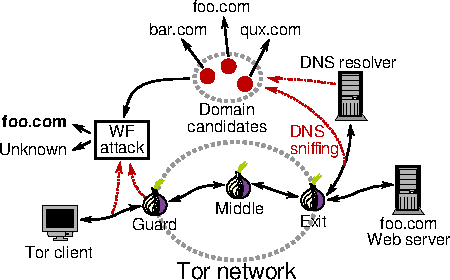
\includegraphics[width=\linewidth]{figures/attack-scenario.pdf}
	\caption{An overview of our correlation attack.  Ingress traffic is
	monitored either by a network-level adversary or the guard relay.  Egress
	traffic is monitored either by a network-level adversary or a DNS server.
	Captured DNS queries then serve as the candidate set for a Website
	fingerprinting attack.}
	\label{fig:attack-scenario}
\end{figure}

\begin{description}
	\item[Ingress sniffing] An attacker must observe traffic that is entering
		the Tor network.  The attacker can operate on the network level, i.e.,
		be a malicious ISP, or an intelligence agency.  In addition, the
		attacker can operate on the relay level, i.e., run a malicious Tor guard
		relay.  Note that in both cases, the attacker can only observe encrypted
		data.  Therefore, packet meta information such as packet lengths and
		directions serve as input to a website fingerprinting
		attack~\cite{Panchenko2016a}.
	\item[Egress sniffing] To observe both ends of the communication, an
		attacker must also observe egress DNS traffic.  We expect the adversary
		to operate on the network level, i.e., be on the path between exit relay
		and a DNS server.  Alternatively, the attacker can run a malicious DNS
		resolver or server.  Note that an attacker may also run an exit relay,
		but in that case she might as well do classical end-to-end correlation.
	\item[WF fingerprinting] We employ a website fingerprinting attack to
		determine if any of the recently observed DNS queries in egress traffic
		could be part of the encrypted ingress traffic.  Note that the DNS query
		itself does not tell us what \emph{page} a user is going to.
\end{description}

\subsection{Egress sniffing -- simulating Tor-exits' DNS traffic}
% TODO: bgre
% the angle is: we have to simulate all DNS traffic from all Tor exits,
% the goal is to convince that we'ev made reasonable assumptions

% phw's numbers extrapolated
% powerlaw, not uniform

% exit caching only (limitation: client-side caching negligible?)
% we ignore caching by having a window of X minutes

% The exit relay maintains its own caching layer around eventdns.c.
% See the code in src/or/dns.c. the DNS cache enforces a minimum TTL of
% 60 seconds and a maximum TTL of 30 minutes (see src/or/dns.c:278). We
% refer to this as Tor's \emph{TTL clipping}.

\subsubsection{DNS 1Mx5 dataset}
% TODO: pulls
% unique domain names are useful + TTL distribution (?)

\subsubsection{A naive website classifier}
% TODO: whomever gets here first :-)
% we only look for unique domain names
% + naive, but already good enough for our purposes
% we note that we can significantly improve attacks by digging deeper
% into TTLs (even with window) and requests
